\subsection{Combined Domain}
We now define a \textit{combined domain} of a given sensitive abstract
domain with the sealed symbolic domain and its one-step execution.
\begin{definition}[Combined Domain]
  A \textit{combined domain} is $\combdom = \sabsdom \times \symbdom$ and its
  concretization function $\combgamma: \combdom \rightarrow \dom$ and join
  operator are defined as follows:
  \begin{align}
    \combgamma((\sabselem, \symbelem)) &= \sgamma(\sabselem) \cup
      \symbgamma(\symbelem)\\
    (\sabselem, \symbelem) \join ({\sabselem}', \symbelem') &= (\sabselem \join
      {\sabselem}', \symbelem \cup \symbelem')
  \end{align}
\end{definition}

Before defining the one-step execution for the combined domain, we introduce
\textit{analysis elements} to easily configure different types of abstract
states in the sensitive abstract domain and the sealed symbolic domain.
\begin{definition}[Analysis Elements]\label{def:aelem}
  An \textit{analysis element} $\aelem \in \aelemset = (\viewset \times \absdom)
  \uplus (\absimapset \times \symbstset)$ is either 1) a pair of a view and an
  abstract state in a sensitive abstract domain $\sabsdom$, or 2) a pair of an
  abstract instantiation map and a sealed symbolic state in a sealed symbolic
  domain $\symbdom$.  Its concretization function $\aelemgamma:
  \aelemset \rightarrow \dom$ is defined as follows:
  \[
    \aelemgamma(\aelem) = \left\{
      \begin{array}{ll}
        \viewmap(\view) \cap \gamma(\abselem) & \text{if} \; (\view, \abselem) = \aelem\\
        \instant{\symbst}{\absimap} & \text{if} \; (\absimap, \symbst) = \aelem\\
      \end{array}
    \right.
  \]
\end{definition}

\begin{figure*}[t]
  \centering
  \begin{subfigure}[t]{0.15\textwidth}
    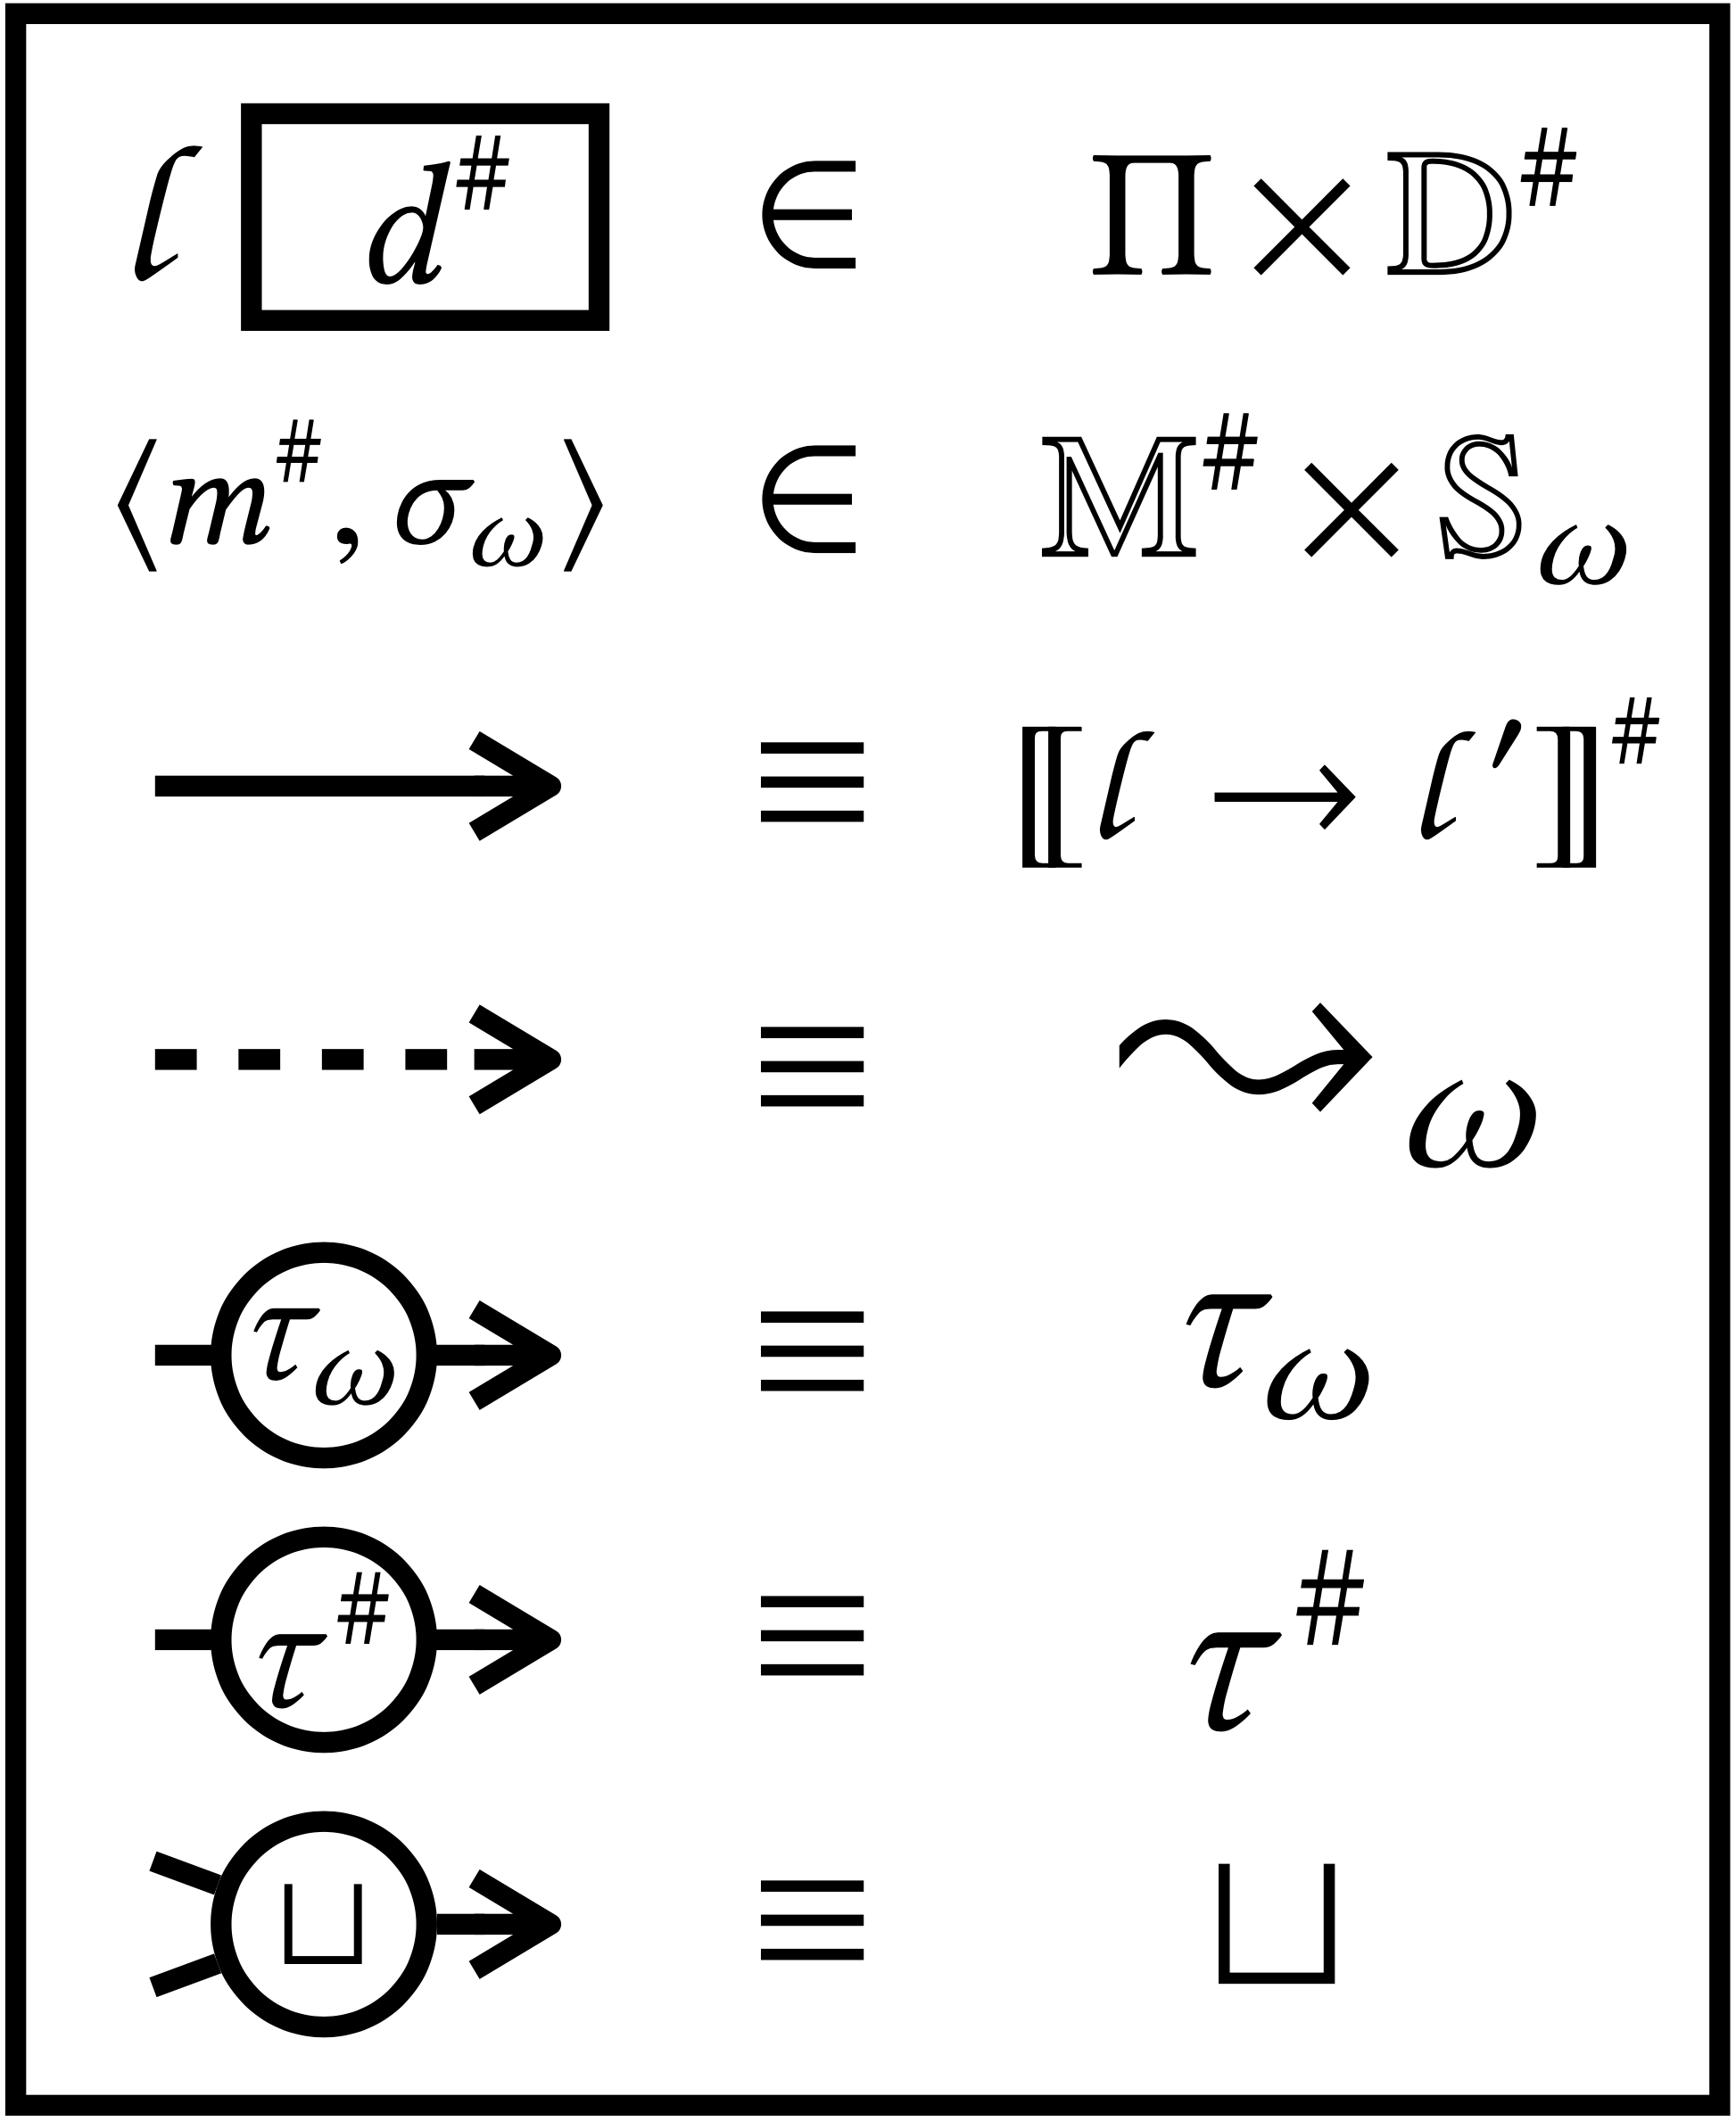
\includegraphics[height=3.2cm]{../img/listing}
    \caption{Notations}
    \label{fig:ds-example1}
  \end{subfigure}
  \quad
  \begin{subfigure}[t]{0.23\textwidth}
    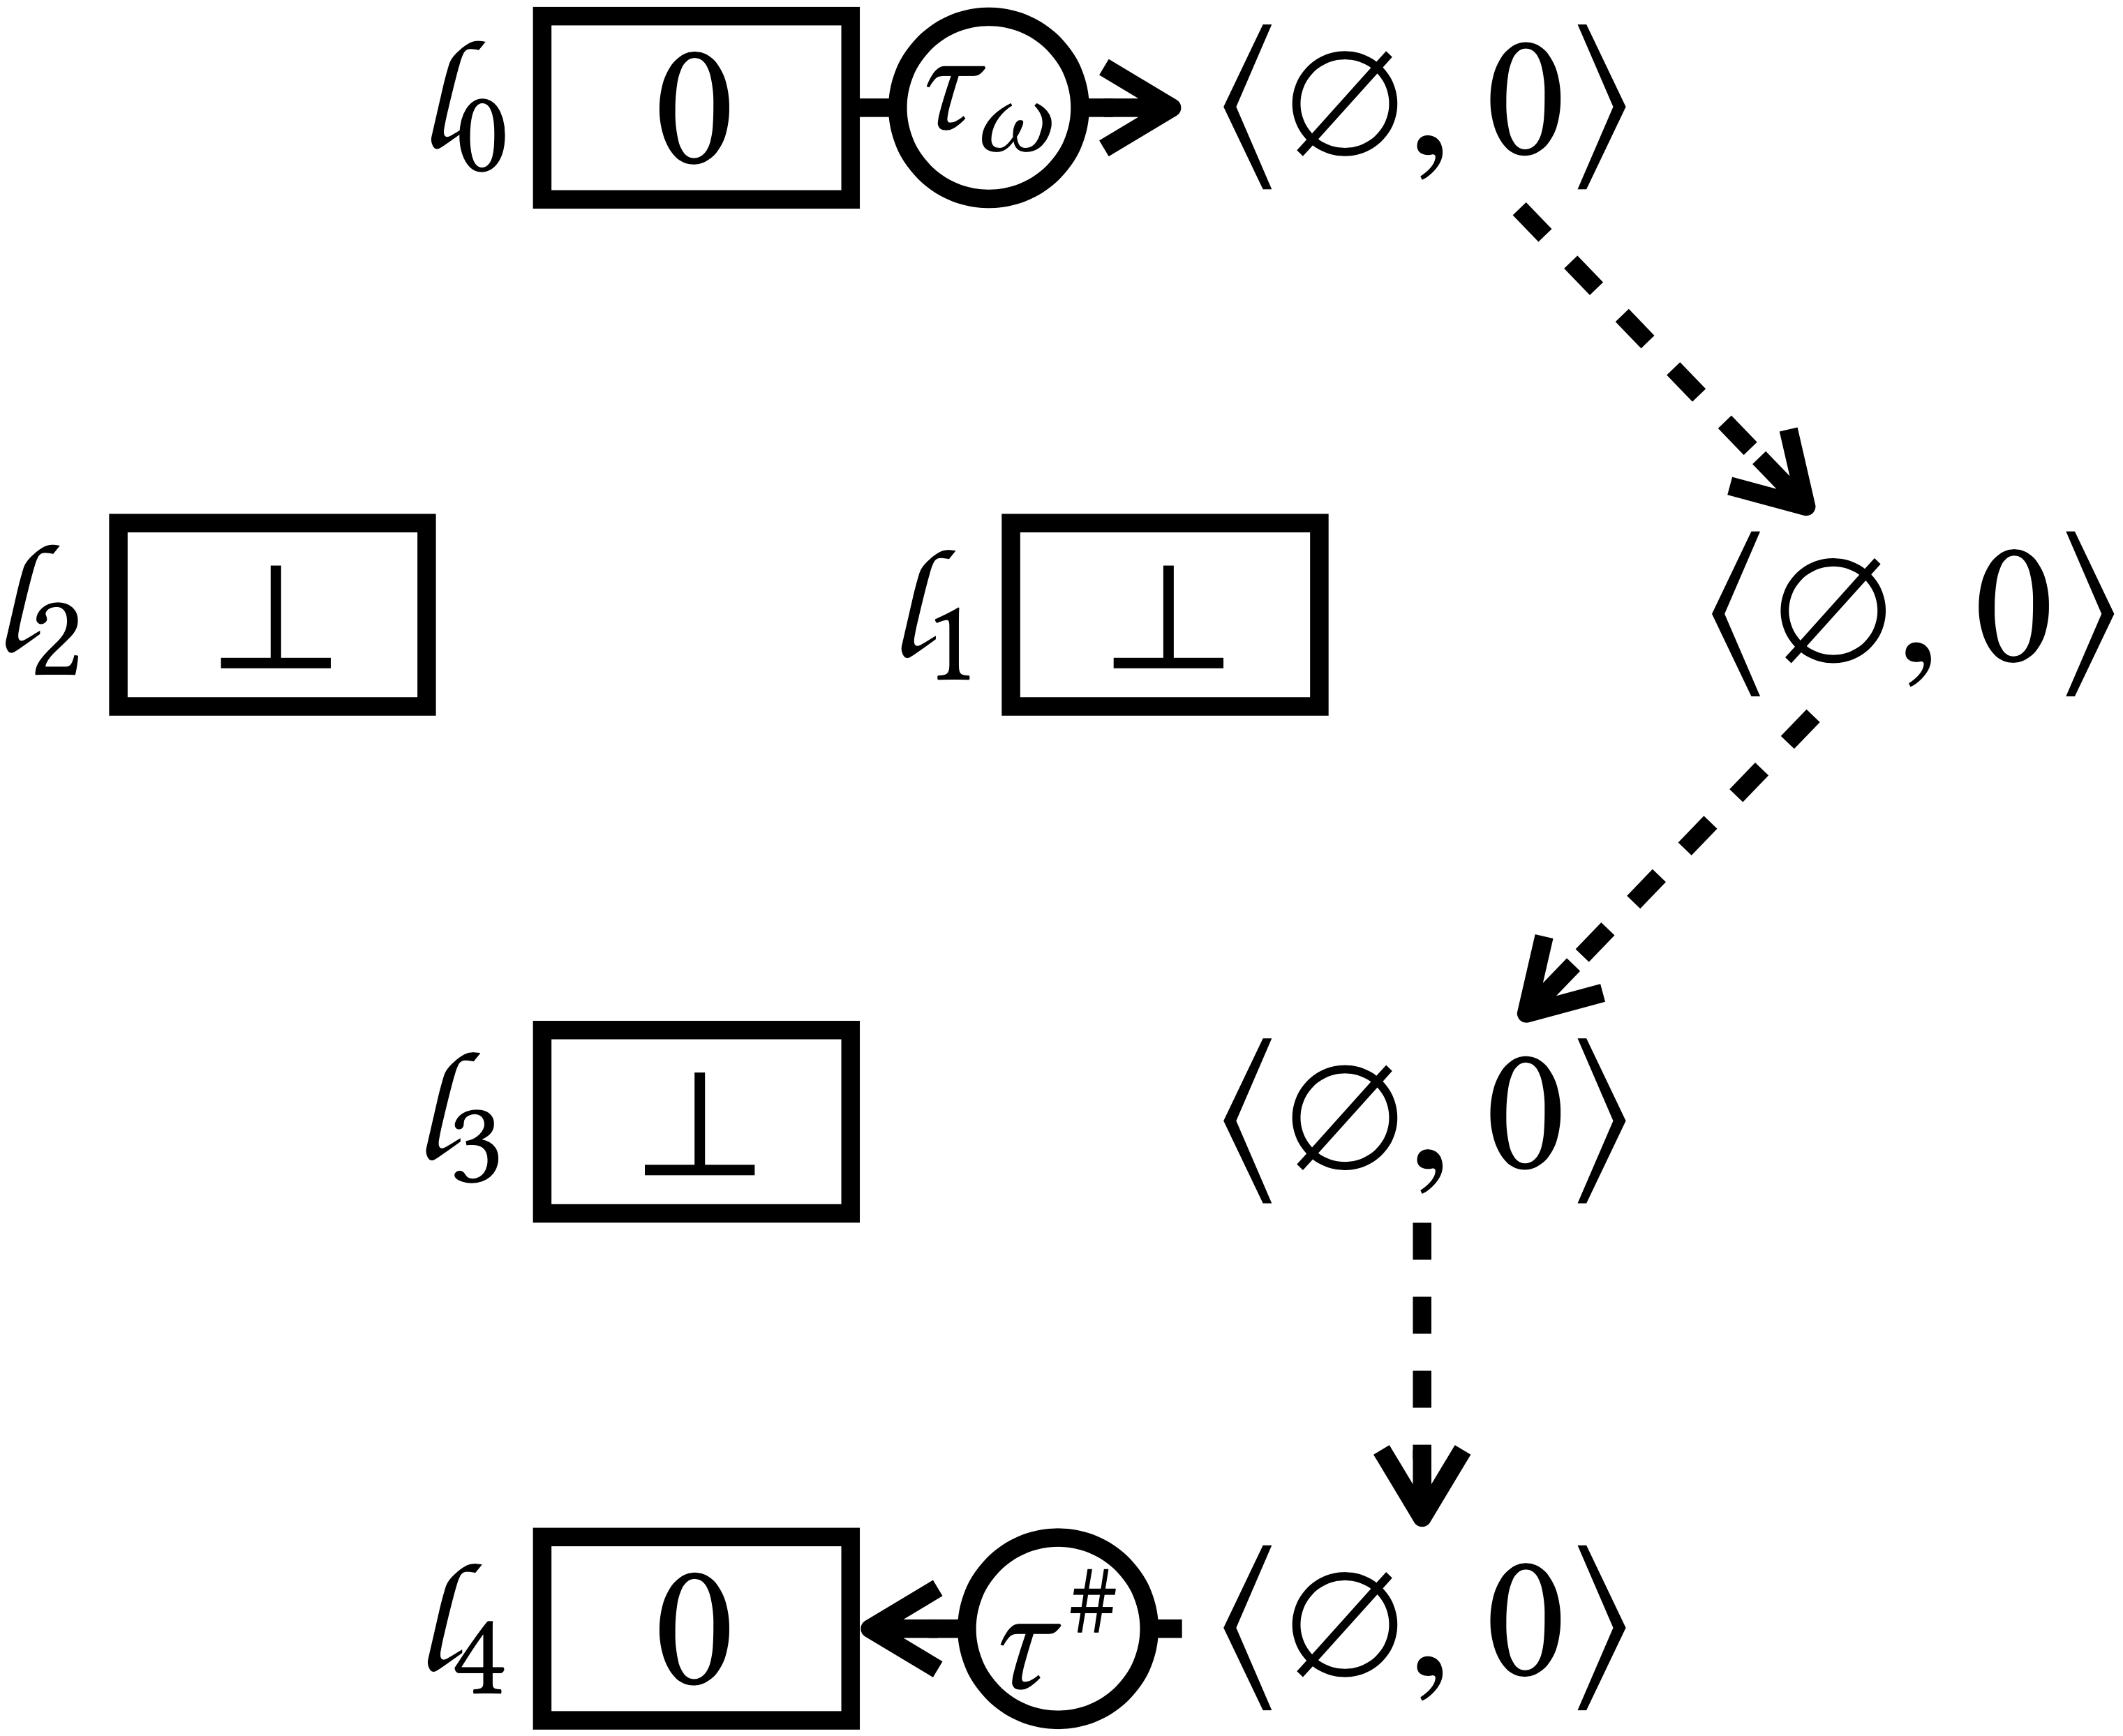
\includegraphics[height=3.2cm]{../img/path-1}
    \caption{$\varx = 0$}
    \label{fig:ds-example2}
  \end{subfigure}
  \begin{subfigure}[t]{0.28\textwidth}
    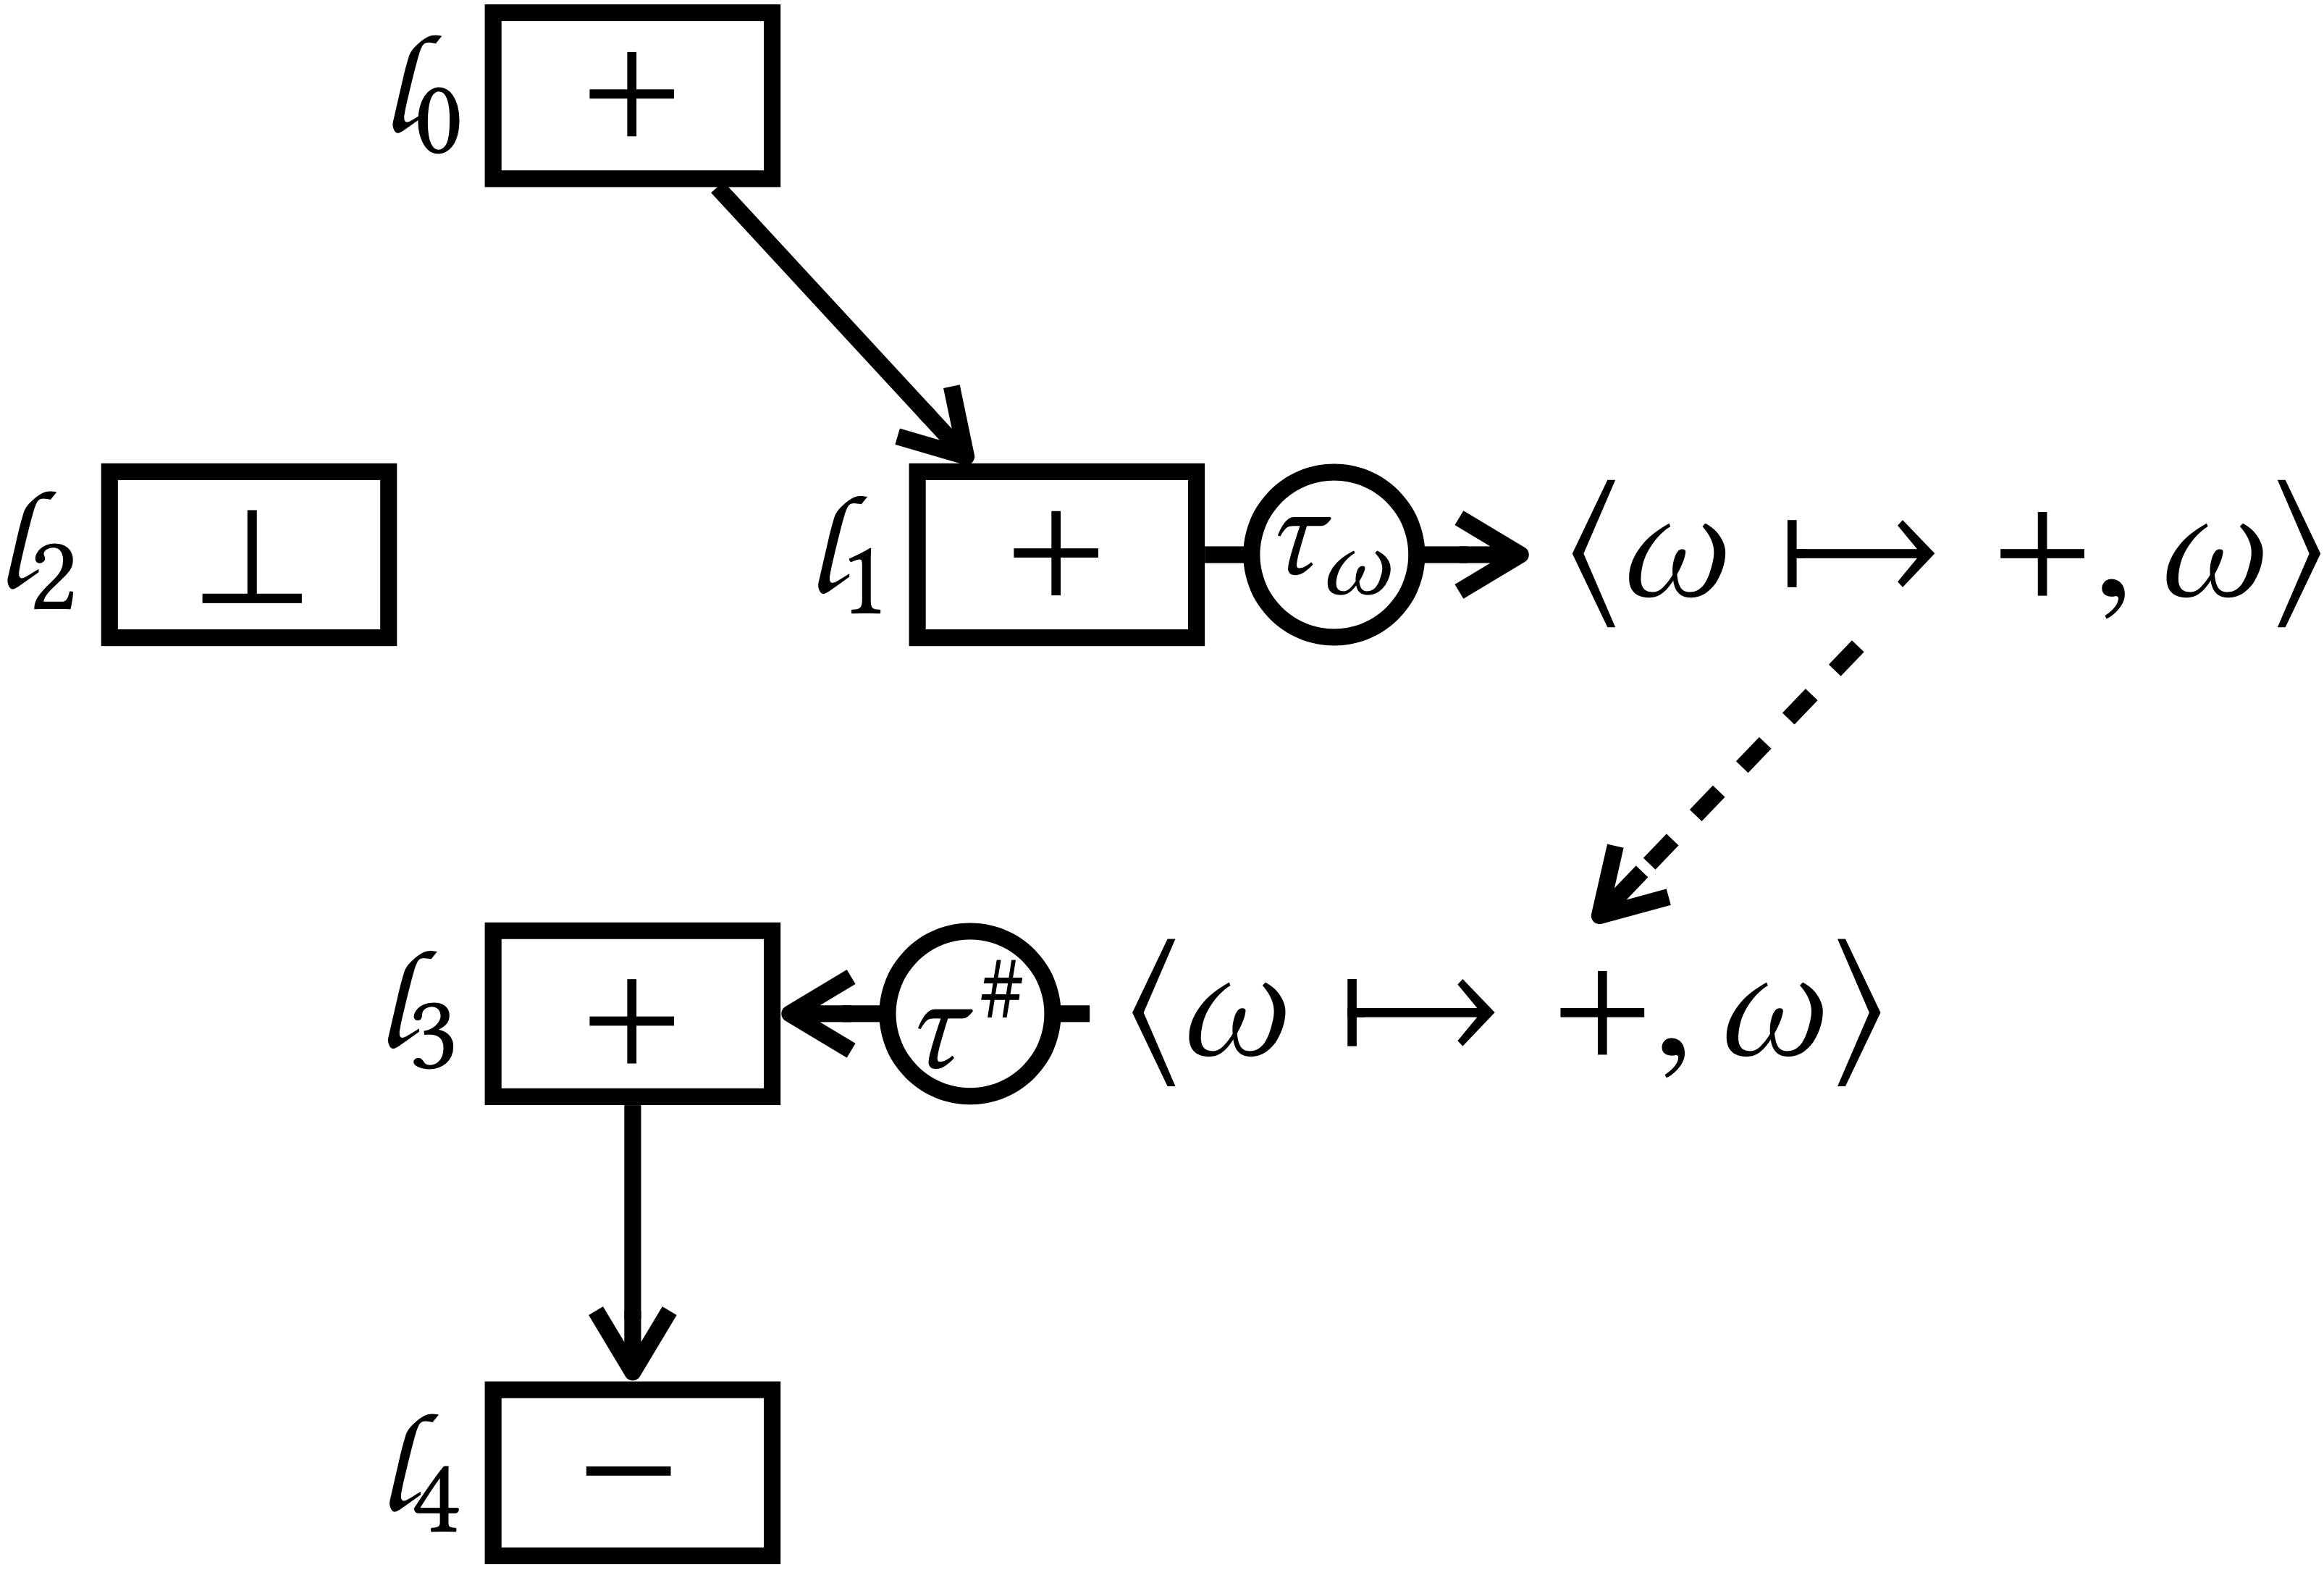
\includegraphics[height=3.2cm]{../img/path-2}
    \caption{$\varx > 0$}
    \label{fig:ds-example3}
  \end{subfigure}
  \begin{subfigure}[t]{0.28\textwidth}
    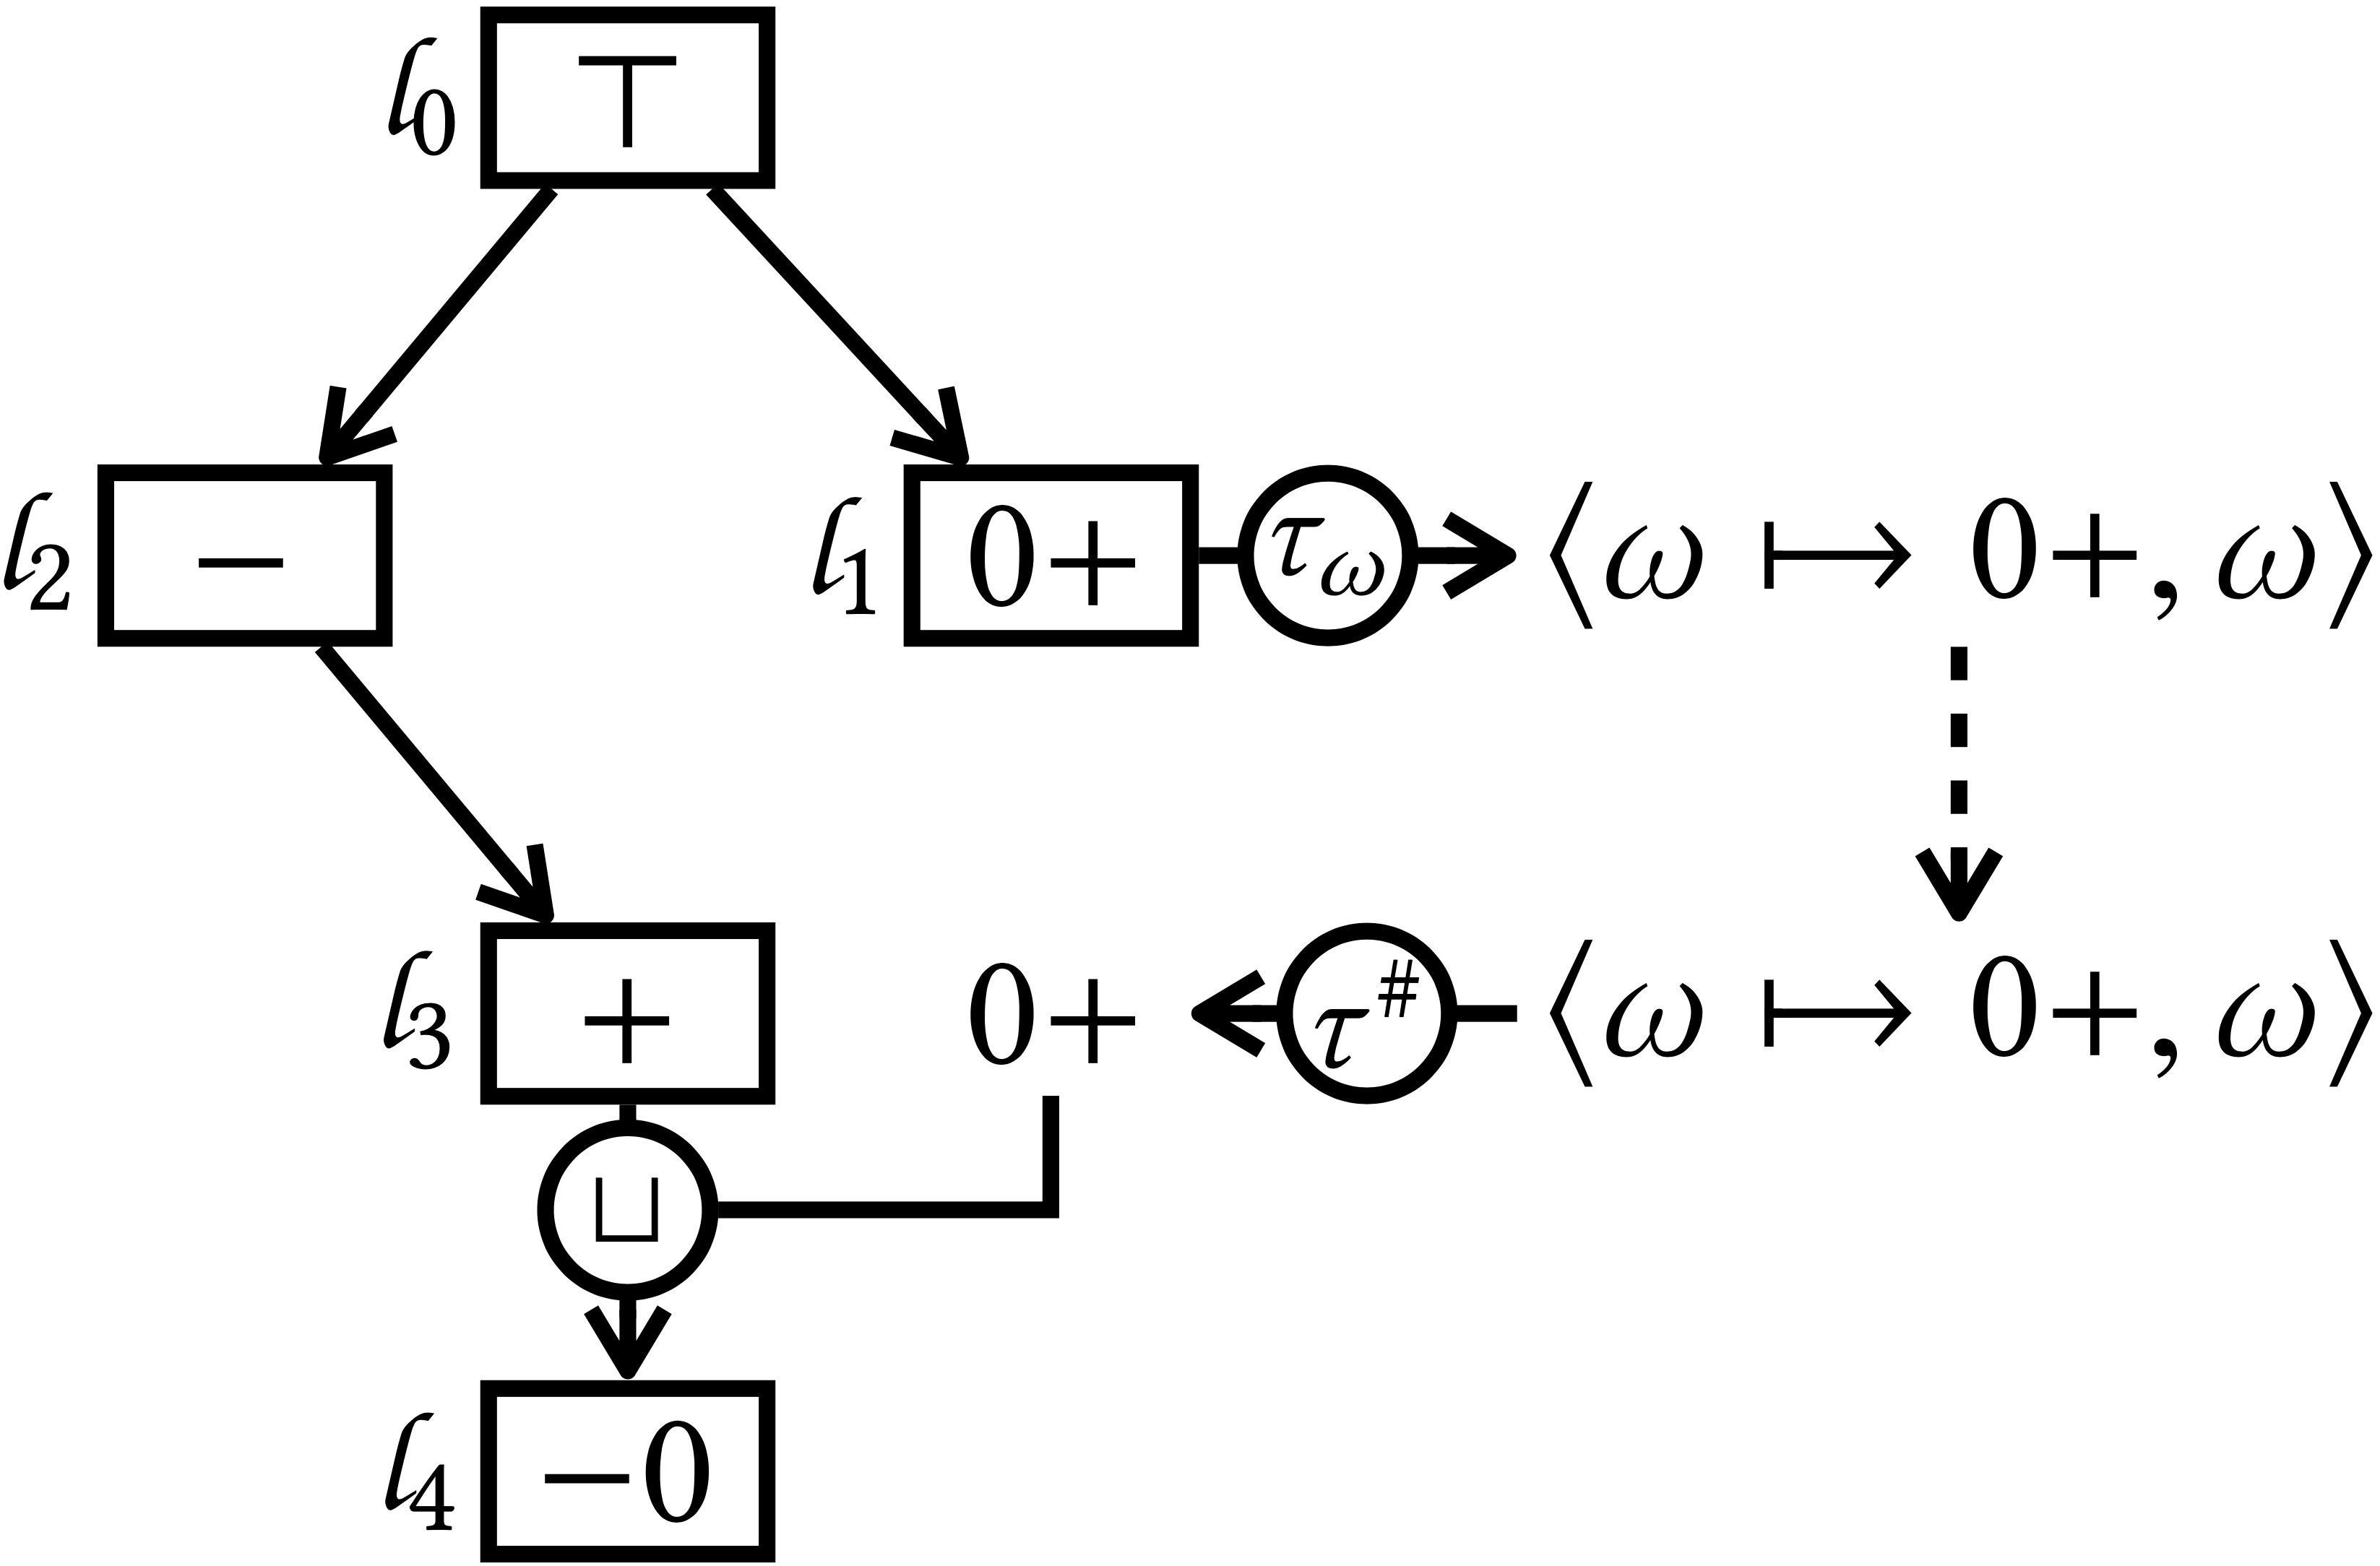
\includegraphics[height=3.2cm]{../img/path-3}
    \caption{$\varx \in \mathbb{N}$}
    \label{fig:ds-example4}
  \end{subfigure}
  \caption{Abstract interpretation using a combined domain for the running
  example with different initial values for $\varx$.}
  \label{fig:ds-examples}
\end{figure*}

Moreover, to freely convert between different kinds of analysis elements, we define two converters:
\begin{align}
  \asconverter & : (\viewset \times \absdom) \hookrightarrow
    (\absimapset \times \symbstset)\\
  \saconverter & : (\viewset \times
    \absdom) \leftarrow (\absimapset \times \symbstset)
\end{align}
While the converter $\saconverter$ is total, the other one $\asconverter$ is
\textit{partial}. Thus, it is possible to convert an analysis element
$(\view, \abselem)$ in a sensitive abstract domain to another analysis element in
a sealed symbolic domain only if the convert $\asconverter$ is defined: $(\view,
\abselem) \in \Dom(\asconverter)$.  In addition, they should convert given
analysis elements without loss of information for all $\aelem \in \aelemset$:
\[
  \asconverter(\aelem) = \aelem' \Rightarrow \left\{
  \begin{array}{l}
    \aelem = \saconverter(\aelem')\\
    \aelemgamma(\aelem) = \aelemgamma(\aelem')\\
  \end{array}
  \right.
\]

Now, we define the \textit{combined one-step execution} $\combstep: \combdom
\rightarrow \combdom$ with two converters $\asconverter$ and $\saconverter$.
It consists of two steps: 1) the \textit{\reformname} step converts
analysis elements if a new sealed symbolic execution starts or an
existing one stops, and 2) the \textit{execution} step performs execution of each
analysis element using the abstract one-step execution $\sabsstep$ in the sensitive
abstract domain and the sealed symbolic one-step execution $\symbstep$ in the sealed
symbolic domain.
\begin{definition}[Combined One-Step Execution]
A \textit{combined one-step execution} $\combstep: \combdom \rightarrow
\combdom$ is define as follows:
  \[
    \combstep(\combelem) = (\sabsstep(\sabselem), \symbstep(\symbelem))
  \]
where $(\sabselem, \symbelem) = \reform(\combelem)$.
\end{definition}

From a given combined state $\combelem$, the $\reform$ function makes analysis elements
and converts them if a new sealed symbolic execution
begins or an existing sealed symbolic execution terminates.
Specifically, for an analysis element $(\view, \abselem)$ in the sensitive abstract domain,
if the converter $\asconverter$ is defined for it, $\reform$ introduces a new sealed symbolic execution
by converting the analysis element to its corresponding one $(\absimap, \symbst) =
\asconverter((\view, \abselem))$ in the sealed symbolic domain.
On the other hand, for an analysis element $(\absimap, \symbst)$ in the sealed symbolic domain,
if it does not have any sealed symbolic states to transit to, $\symbst \symbtrans \excst$,
the sealed symbolic execution for $(\absimap, \symbst)$ terminates;
It converts the analysis element to its corresponding one $(\view, \abselem) =
\saconverter((\absimap, \symbst))$ in the sensitive abstract domain and
merges the current abstract state stored in the view $\view$ with $\abselem$.

To formally define the $\reform$ function, we first define a $\areform$ function
for analysis elements using two converters.
\begin{definition}[$\areform$]\label{def:areform}
  The function $\areform: \aelemset \rightarrow \aelemset$ for analysis elements
  is defined as follows:
  \[
    \areform(\aelem) = \left\{
      \begin{array}{ll}
        \asconverter(\aelem)
        & \text{if} \; \aelem = (\view, \abselem) \wedge \aelem \in
        \Dom(\asconverter)\\
        \saconverter(\aelem)
        & \text{if} \; \aelem = (\absimap, \symbst) \wedge \symbst \symbtrans
        \bot\\
        \aelem
        & \text{Otherwise}
      \end{array}
    \right.
  \]
\end{definition}
\begin{definition}[$\reform$]\label{def:reform}
  The \reformname function $\reform: \combdom \rightarrow \combdom$ for combined
  states is defined as follows:
  \[
    \reform((\sabselem, \symbelem)) = \left(
      \lambda \view. \bigjoin \{ \abselem \!\mid\! (\view, \abselem) \in E \},
      E \cap (\absimapset \times \symbstset)
    \right)
  \]
  where
  \[
    E = \dot{\areform}(\{ (\view, \sabselem(\view)) \mid \view \in \viewset \} \cup \symbelem)
  \]
and the dot notation $\dot{f}$ denotes the element-wise extended function of a
function $f$.
\end{definition}


\subsection{Examples}
Now, we show examples of abstract interpretation with a combined domain.
Figure~\ref{fig:ds-examples} depicts the flow of analysis for the running
example in Figure~\ref{fig:running-example} with three different initial sets of
values for the variable $\varx$.  In this example, we use the abstract domain
$\{ -, 0, + \}$ for integers stored in $\varx$ as introduced in
Section~\ref{sec:ai}, and the \textit{flow sensitivity} that utilizes the
labels of states as their views as introduced in Section~\ref{sec:sens}.
For brevity, we use concatenation of abstract values so that
$-0$ denotes the set $\{ -, 0 \}$.

Figure~\ref{fig:ds-examples}(a) presents notations used in each graph. A solid
box denotes an analysis element that is a pair of a label $\lab$ and an abstract
state $\abselem$.  A pair enclosed by angle brackets denotes an analysis
element that is a pair of an abstract instantiation map $\absimap$ and a sealed
symbolic state $\symbst$.  In fact, the sealed symbolic state part (right) of
each pair in graphs contains only the value of the variable of $\varx$ without
its label.  For brevity, we represent its label by locating it next to
a node with its label.  A solid line is a view transition
$\viewtrans{\lab}{\lab'}$ from a label $\lab$ to another one $\lab'$.  A dotted
line is a sealed symbolic transition $\symbtrans$.  Three solid lines with
circled labels denote two converters $\saconverter$, $\asconverter$ and the join
operator $\join$.

Figure~\ref{fig:ds-examples}(b) shows the analysis with the combined domain when
the initial value of $\varx$ is $0$.  First, in the \reformname step,
the converter $\asconverter$ converts the analysis element $(\lab_0, 0)$ to
another analysis element $\langle \varnothing, 0 \rangle$ with the label
$\lab_0$.  It does not introduce any sealed symbolic values because
the value represents only a single value.  Until the end of the program, the
sealed symbolic execution from $\langle \varnothing, 0 \rangle$ successfully
continues.  Because there is no more possible symbolic transition for the
symbolic state $\langle \varnothing, 0 \rangle$ with the label $\lab_4$,
it is converted to $(\lab_4, 0)$ via the converter $\saconverter$.

Instead of a single value, assume that the initial value of $\varx$ is one of
any positive integers.  Figure~\ref{fig:ds-examples}(c) describes the analysis
flow for the case.  The initial abstract value at the label $\lab_0$ is
$+$ and it is impossible to convert it to any sealed symbolic values because the
next program statement requires the actual value stored in the variable $\varx$
for the branch condition $\varx \geq 0$.  Thus, it performs view transition
$\viewtrans{\lab_0}{\lab_1}$ from the label $\lab_0$ to another one $\lab_1$ for
the abstract value $+$ and the result is also $+$.  Now, the analysis element
$(\lab_1, +)$ can be converted to $\langle \symb \mapsto +, \symb \rangle$
with the label $\lab_1$.  This sealed symbolic execution step terminates in the
label $\lab_3$ because the next statement is $\varx = -\varx$ and the negation
operator requires the actual value of $\varx$.  It is converted to $(\lab_3, +)$ via $\saconverter$,
performs the view transition, and results in $(\lab_4, -)$.

For the last case, we assume that all integers are possible for the initial
value of the variable $\varx$ as described in Figure~\ref{fig:ds-examples}(d).
While it reaches the false branch in the label $\lab_2$ unlike previous cases,
it cannot perform dynamic shortcuts because the statement in the false
branch is $\varx = -\varx$, which requires the actual value of $\varx$.
At the label $\lab_3$, there are two analysis
elements: 1) $(\lab_3, +)$ introduced by the view transition from the label $\lab_2$
with $-$, and 2) $\langle \symb \mapsto 0+, \symb \rangle$ with $\lab_3$
introduced by sealed symbolic execution started at $\lab_1$.  Since it
is not possible to perform sealed symbolic execution for both elements, the
second one is converted to $(\lab_3, 0+)$ and merged with $+$ at $\lab_3$ via the
join operator $\join$.  Finally, the view transition
$\viewtrans{\lab_3}{\lab_4}$ from $\lab_3$ to $\lab_4$ is performed to the
merged abstract state $0+$ and the result is $-0$.

\subsection{Soundness and Termination}
The converter $\asconverter$ and the sealed symbolic transition $\symbtrans$ are
keys to configure the introduction and termination of sealed symbolic
execution.  To ensure the \textit{soundness} and \textit{termination} of an
abstract interpretation defined with a combined domain of a sensitive abstract
domain and a sealed symbolic domain, the following conditions should hold.

\begin{theorem}[Soundness and Termination]\label{theorem:shortcut}
An abstract interpretation with dynamic shortcuts is \textbf{sound} and
\textbf{terminates} in a finite time if:
  \begin{itemize}
    \item the abstract transfer function $\abstransfer$ is sound,
    \item the sensitive abstract domain $\sabsdom$ has a finite height,
    \item the sealed symbolic transition $\symbtrans$ is valid, and
    \item there exists $N < \infty$ such that
      \[
        \forall \aelem \in \aelemset. \; \asconverter(\aelem) = (\absimap,
        \symbst) \Rightarrow \symbst
        \symbtrans^k \excst \wedge 1 < k \leq N
      \]
  \end{itemize}
\end{theorem}

To formally prove Theorem~\ref{theorem:shortcut}, we assume that its all
conditions are hold and rephrase the \textit{soundness} as
Theorem~\ref{theorem:soundness} and \textit{termination} as
Theorem~\ref{theorem:termination}.

\subsubsection{Soundness}

\begin{theorem}[Soundness]\label{theorem:soundness}
  The abstract interpretation using the combined domain $\combdom$ is
  \textbf{sound} if
  \begin{equation}\label{equ:sound-join}
    \forall \combelem_0, \combelem_1 \in \combdom. \; \combgamma(\combelem_0) \cup
    \combgamma(\combelem_1) \subseteq \combgamma(\combelem_0 \join \combelem_1)
  \end{equation}
  \begin{equation}\label{equ:sound-combstep}
    \forall \combelem \in \combdom. \; \step \circ \combgamma(\combelem) \subseteq
    \combgamma \circ \combstep(\combelem)\\
  \end{equation}
\end{theorem}
\begin{proof}
  First, we prove that the abstract transfer function $\combtransfer: \combdom
  \rightarrow \combdom$ defined as $\combtransfer(\combelem) = \combelem \join
  \combstep(\combelem)$ is sound
  \[
    \begin{array}{rcll}
      \transfer \circ \combgamma(\combelem)
      &=& \combgamma(\combelem) \cup \step \circ \combgamma(\combelem)\\
      &\subseteq& \combgamma(\combelem) \cup \combgamma \circ \combstep(\combelem)
      & (\because \; \text{condition~(\ref{equ:sound-combstep})})\\
      &\subseteq& \combgamma(\combelem \join \combstep(\combelem))
      & (\because \; \text{condition~(\ref{equ:sound-join})})\\
      &=& \combgamma \circ \combtransfer(\combelem)\\
    \end{array}
  \]
  Then, the abstract semantics $\combsem{\prog} = \underset{n \rightarrow
  \infty}{\lim}{(\combtransfer)^n(\icombelem)} $ is also sound because it is
  defined with a sound abstract transfer function $\combtransfer$ using the
  combined one-step execution $\combstep$.
\end{proof}

Now, we should show that two conditions about the soundness of the join
operator (\ref{equ:sound-join}) and the soundness of the combined one-step
execution (\ref{equ:sound-combstep}) in Theorem~\ref{theorem:soundness} hold.

First, we prove the soundness of the join operator (\ref{equ:sound-join}) in
Lemma~\ref{lemma:sound-join}.
\begin{lemma}[Soundness of $\join$]\label{lemma:sound-join}
  \[
    \forall \combelem_0, \combelem_1 \in \combdom. \; \combgamma(\combelem_0) \cup
    \combgamma(\combelem_1) \subseteq \combgamma(\combelem_0 \join \combelem_1)
  \]
\end{lemma}
\begin{proof}
  \[
    \begin{array}{cl}
      \multicolumn{2}{l}{
        \combgamma((\sabselem, \symbelem)) \cup \combgamma((\sabselem', \symbelem'))
      }\\
      =& \sgamma(\sabselem) \cup \symbgamma(\symbelem)
      \cup \sgamma(\sabselem') \cup \symbgamma(\symbelem')\\
      =& (\sgamma(\sabselem)\cup \sgamma(\sabselem'))
      \cup (\symbgamma(\symbelem) \cup \symbgamma(\symbelem'))\\
      \subseteq& \sgamma(\sabselem \join \sabselem')
      \cup (\symbgamma(\symbelem) \cup \symbgamma(\symbelem'))\\
      & \multicolumn{1}{r}{(\because \; \sabsdom \; \text{is sound})}\\
      =& \sgamma(\sabselem \join \sabselem')
      \cup \symbgamma(\symbelem \cup \symbelem')\\
      =& \combgamma((\sabselem \join \sabselem', \symbelem \cup \symbelem'))\\
      =& \combgamma((\sabselem, \symbelem) \join (\sabselem', \symbelem'))\\
    \end{array}
  \]
\end{proof}

For the condition (\ref{equ:sound-combstep}), we first prove two properties of the
$\reform$ function in Lemma~\ref{lemma:reform}.  Using the properties, we prove
the soundness of the sealed symbolic one-step execution in
Lemma~\ref{lemma:sound-symbstep}.  Finally, we prove the soundness of the
combined one-step execution (\ref{equ:sound-combstep}) in
Lemma~\ref{lemma:sound-combstep}.

\begin{lemma}[Properties of $\reform$]\label{lemma:reform}
  For a given combined state $\combelem \in \combdom$, the $\reform$ function
  satisfies the following two properties:
  \begin{itemize}
    \item $\combgamma(\combelem) \subseteq \combgamma \circ \reform(\combelem)$
    \item $\forall (\absimap, \symbst) \in \symbelem. \; \exists \symbst' \in
      \symbstset.  \; \text{s.t.} \; \symbst \symbtrans \symbst'$
  \end{itemize}
  where $(\sabselem, \symbelem) = \reform(\combelem)$
\end{lemma}
\begin{proof}
  \[
    \fbox{$\combgamma(\combelem) \subseteq \combgamma \circ \reform(\combelem)$}
  \]
  \[
    \begin{array}{cl}
      \multicolumn{2}{l}{\combgamma((\sabselem, \symbelem))}\\
      =& \sgamma(\sabselem) \cup \symbgamma(\symbelem)\\

      =& \left( \underset{\view \in \viewset}{\bigcup} {\viewmap(\view) \cap
      \gamma \circ \sabselem(\view)} \right) \cup \left( \underset{(\absimap,
      \symbst) \in \symbelem}{\bigcup} \instant{\symbst}{\absimap} \right) \\

      =& \left( \underset{\view \in \viewset}{\bigcup} \aelemgamma((\view,
      \sabselem(\view))) \right) \cup \left( \underset{(\absimap, \symbst) \in
      \symbelem}{\bigcup} \aelemgamma((\absimap, \symbst)) \right) \\

      =& \dot\aelemgamma(\{ (\view, \sabselem(\view)) \mid \view \in \viewset \}
      \cup \symbelem)\\

      =& \dot\aelemgamma(\dot{\areform}(\{ (\view, \sabselem(\view)) \mid \view
      \in \viewset \} \cup \symbelem))\\

       & \multicolumn{1}{r}{\because \; (\text{Trivially,} \; \forall \aelem \in
       \aelemset.  \; \aelemgamma(\aelem) = \aelemgamma \circ \areform(\aelem))}\\

      =& \dot\aelemgamma(E)\\
       & \multicolumn{1}{r}{\because \; (\text{See the definition of $E$ in
       Definition~\ref{def:reform}})}\\
    \end{array}
  \]
  \[
    \begin{array}{cl}
      =& \left( \underset{(\view, \abselem) \in E}{\bigcup} \aelemgamma((\view,
      \abselem)) \right) \cup \left( \underset{(\absimap, \symbst) \in
      E}{\bigcup} \aelemgamma((\absimap, \symbst)) \right)\\

      =& \left( \underset{(\view, \abselem) \in E}{\bigcup} \viewmap(\view) \cap
      \gamma(\abselem) \right) \cup \left( \underset{(\absimap, \symbst) \in
      E}{\bigcup} \instant{\symbst}{\absimap} \right)\\

      =& \left( \underset{\view \in \viewset}{\bigcup} { \underset{(\view,
      \abselem) \in E}{\bigcup} \viewmap(\view) \cap \gamma(\abselem) } \right)
      \cup \left( \underset{(\absimap, \symbst) \in E}{\bigcup}
      \instant{\symbst}{\absimap} \right)\\

      =& \left( \underset{\view \in \viewset}{\bigcup} {\viewmap(\view) \cap
        \left(\underset{(\view, \abselem) \in
      E}{\bigcup}{\gamma(\abselem)}\right)} \right) \cup \left(
      \underset{(\absimap, \symbst) \in E}{\bigcup} \instant{\symbst}{\absimap}
      \right)\\

      \subseteq& \left( \underset{\view \in \viewset}{\bigcup} {\viewmap(\view)
        \cap \gamma\left( \underset{(\view, \abselem) \in E}{\bigjoin}\abselem
      \right)} \right) \cup \left( \underset{(\absimap, \symbst) \in E}{\bigcup}
      \instant{\symbst}{\absimap} \right)\\

      =& \sgamma\left( \lambda \view. \underset{(\view, \abselem) \in
      E}{\bigjoin}\abselem \right) \cup \symbgamma(E \cap (\absimapset \times
      \symbstset))\\

      =& \combgamma\left( \lambda \view. \underset{(\view, \abselem) \in
      E}{\bigjoin}\abselem, E \cap (\absimapset \times \symbstset) \right)\\

      =& \combgamma \circ \reform((\sabselem, \symbelem))
    \end{array}
  \]
  \[\]
  \[
    \fbox{$\forall (\absimap, \symbst) \in \symbelem. \; \exists \symbst' \in
    \symbstset.  \; \text{s.t.} \; \symbst \symbtrans \symbst'$}
  \]

  For a given $(\absimap, \symbst) \in \symbelem$, there exists an analysis
  element $\aelem \in \aelemset$ such that $\areform(\aelem) = (\absimap,
  \symbst)$.  According to the definition of $\areform$ in
  Definition~\ref{def:areform}, there are two possible cases: $\aelem =
  (\absimap, \symbst) \wedge \exists \symbst' \in \symbstset. \; \text{s.t} \;
  \symbst \symbtrans \symbst'$ or $\aelem = (\view, \abselem) \wedge \aelem \in
  \Dom(\asconverter)$. We separately consider those two cases:
  \begin{itemize}
    \item $\aelem = (\absimap, \symbst) \wedge \exists \symbst' \in \symbstset.
      \; \text{s.t} \; \symbst \symbtrans \symbst'$\\
        By definition, $\exists \symbst' \in \symbstset.  \; \text{s.t} \;
        \symbst \symbtrans \symbst'$
    \item $\aelem = (\view, \abselem) \wedge \aelem \in \Dom(\asconverter)$\\
      By the condition~\ref{equ:asc-cond} in the Theorem~\ref{theorem:shortcut},\\
      $\exists k > 1. \symbst \symbtrans^k \excst$.  Thus, $\exists \symbst' \in
      \symbstset.  \; \text{s.t} \; \symbst \symbtrans \symbst'$
  \end{itemize}
\end{proof}

\begin{lemma}[Soundness of $\symbstep$]\label{lemma:sound-symbstep}
  The sealed symbolic one-step execution $\symbstep$ is sound:
  \[
    \step \circ \symbgamma(\symbelem) \subseteq
    \symbgamma \circ \symbstep(\symbelem)\\
  \]
\end{lemma}
\begin{proof}
  \[
    \begin{array}{cl}
      \multicolumn{2}{l}{\step \circ \symbgamma(\symbelem)}\\
      =& \step(\bigcup \{ \instant{\symbst}{\absimap} \mid (\absimap, \symbst) \in
      \symbelem\})\\
      =& \{ \st' \mid (\absimap, \symbst) \in \symbelem \wedge \st \in
      \instant{\symbst}{\absimap} \wedge \st \trans \st'\})\\
      =& \{ \st' \mid (\absimap, \symbst) \in \symbelem \wedge \imap \in
      \imapgamma(\absimap) \wedge \instant{\symbst}{\imap} \trans \st'\})\\
      =& \{ \st' \mid (\absimap, \symbst) \in \symbelem \wedge \imap \in
      \imapgamma(\absimap) \wedge \instant{\symbst}{\imap} \trans \st'\\
       & \phantom{\{ \st' \mid (\absimap, \symbst) \in \symbelem \wedge \imap \in
      \imapgamma(\absimap)} \wedge \symbst \symbtrans \symbst' \})\\
       & \multicolumn{1}{r}{(\because \; \text{Second property in
       Lemma~ref{lemma:reform}})}\\
      =& \{ \instant{\symbst'}{\imap} \mid (\absimap, \symbst)
      \in \symbelem \wedge \imap \in \imapgamma(\absimap) \wedge \symbst
      \symbtrans \symbst'\}\\
      & \multicolumn{1}{r}{(\because \; \text{Validity of} \; \symbtrans)}\\
      =& \bigcup \{ \instant{\symbst'}{\absimap} \mid (\absimap, \symbst)
      \in \symbelem \wedge \symbst \symbtrans \symbst' \}\\
      =& \symbgamma(\{ (\absimap, \symbst') \mid (\absimap, \symbst)
      \in \symbelem \wedge \symbst \symbtrans \symbst' \})\\
      =& \symbgamma \circ \symbstep(\symbelem)\\
    \end{array}
  \]
\end{proof}

\begin{lemma}[Soundness of $\combstep$]\label{lemma:sound-combstep}
  The combined one-step execution $\combstep$ is sound:
  \[
    \forall \combelem \in \combdom. \; \step \circ \combgamma(\combelem) \subseteq
    \combgamma \circ \combstep(\combelem)\\
  \]
\end{lemma}
\begin{proof}
  \[
    \begin{array}{cl}
      \multicolumn{2}{l}{
        \step \circ \combgamma(\combelem)
      }\\
      \subseteq& \step \circ \combgamma((\sabselem, \symbelem))\\
       & \multicolumn{1}{r}{(\because \; \text{First property in
       Lemma~\ref{lemma:reform}}}\\
       & \multicolumn{1}{r}{\text{where} \; (\sabselem, \symbelem)
       = \reform(\combelem).)}\\

      =& \step(\sgamma(\sabselem) \cup \symbgamma(\symbelem))\\
      =& \step(\sgamma(\sabselem)) \cup \step(\symbgamma(\symbelem))\\
      \subseteq& \sgamma \circ \sabsstep(\sabselem) \cup \step(\symbgamma(\symbelem))\\
      & \multicolumn{1}{r}{(\because \; \sabsstep \; \text{is sound.})}\\
      \subseteq& \sgamma \circ \sabsstep(\sabselem) \cup \symbgamma \circ
      \symbstep((\symbelem))\\
               & \multicolumn{1}{r}{(\because \; \text{and
               Lemma~\ref{lemma:sound-symbstep}})}\\
      =& \combgamma((\sabsstep(\sabselem), \symbstep(\symbelem)))\\
      =& \combgamma \circ \combstep(\combelem)\\
    \end{array}
  \]
\end{proof}


\subsection{Termination}

Before proving the termination of the abstract interpretation using the combined
domain $\combdom$, we define several notations. The initial abstract state
$\icombelem = (\isabselem, \varnothing)$ is pair of the initial abstract state of
the sensitive abstract domain $\sabsdom$ and an empty set. For each iteration $i
\geq 0$, we define the $i$-th result of abstract interpretation
$\combtransfer^i(\icombelem) = \combelem^i = (\sabselem^i, \symbelem^i)$ and the
\textit{difference set} $\diffset_i = \symbelem^{i+1} \setminus \symbelem^i$.
For simplicity, we define $\diffset_i$ as $\varnothing$ for $i < 0$.  Moreover, we
define a lifted version of sealed symbolic relation $\liftsymbtrans \subseteq
(\absimapset \times \symbstset) \times (\absimapset \times \symbstset)$ as
follows:
\[
  (\absimap, \symbst) \liftsymbtrans (\absimap, \symbst') \Leftrightarrow
  \symbst \symbtrans \symbst'
\]
Using the lifted relation, we define the \textit{time to live (TTL)} function of
symbolic states $\ttl_i: \diffset_i \rightarrow \numset$ for each iteration $i
\geq 0$ as follows:
\begin{definition}[TTL Function]
  \[
    \begin{array}{c}
      \ttl_i(\symbaelem) = \left \{
      \begin{array}{l}
        N - 1 \;\; ( \text{if} \; D = \varnothing)\\
        \text{min}(\dot\ttl_{i-1}(D)) - 1
        \;\; ( \text{otherwise})
      \end{array}
      \right. \\
      \\
      \text{where} \; D =
      \{\symbaelem' \in \diffset_{i-1} \mid \symbaelem' \liftsymbtrans \symbaelem\}
    \end{array}
  \]
\end{definition}

Based on the notations, we formally prove the termination property as folows:
\begin{theorem}[Termination]\label{theorem:termination}
  The abstract interpretation using the combined domain $\combdom$
  \textbf{terminates} in a finite time if
  \begin{equation}\label{equ:termination-sai}
    \exists n. \; \forall m \geq n. \; \sabselem^m = \sabselem^n
  \end{equation}
  \begin{equation}\label{equ:bounded-ttl}
    \forall i \geq 0. \; \forall \symbaelem \in \diffset_i. \;
    0 < \ttl_i(\symbaelem) < N
  \end{equation}
  \begin{equation}\label{equ:dec-ttl}
    \begin{array}{c}
      \forall i > 0. \; \sabselem^{i-1} = \sabselem^i \Rightarrow\\
      \sup(\dot \ttl_i(\diffset_i)) \leq \sup(\dot \ttl_{i-1}(\diffset_{i-1})) - 1
    \end{array}
  \end{equation}
\end{theorem}

\begin{proof}
  By the condition (\ref{equ:termination-sai}), there exists $n \in \numset$
  such that $\sabselem^m = \sabselem^n$ for all $m \geq n$.  By the condition
  (\ref{equ:bounded-ttl}), the TTL of each symbolic state in $\diffset_n$ is
  bounded by $N$:
  \[
    \sup(\dot \ttl_n(\diffset_n)) < N
  \].
  Then, the upper bound of TTL for symbolic states in each difference set after
  the $n-$th iteration is decreased by the condition (\ref{equ:dec-ttl}):
  \[
    \forall i > 0. \; \sup(\dot \ttl_{n+i}(\diffset_{n+i})) \leq \sup(\dot
    \ttl_{n+i-1}(\diffset_{n+i-1})) - 1
  \].
  which implies that
  \[
    \sup(\dot \ttl_{n+i}(\diffset_{n+i})) \leq \sup(\dot \ttl_n(\diffset_n)) - i < N - i
  \]
  Therefore, for $j \geq N$,
  \[
    \sup(\dot \ttl_{n+j}(\diffset_{n+j})) < N - j \leq 0
  \]
  Notice that again by the condition (\ref{equ:bounded-ttl}),
  \[
    inf(\dot \ttl_{n+j}(\diffset_{n+j})) > 0
  \]
  meaning that
  \[
    inf(\dot \ttl_{n+j}(\diffset_{n+j})) > \sup(\dot \ttl_{n+j}(\diffset_{n+j}))
  \]
  which implies $\diffset_{n+j} = \varnothing$ and $\symbelem^{n+j+1} =
  \symbelem^{n+j}$.
  Therefore, for all $m \geq n + N$,
  \[
    \sabselem^m = \sabselem^{n+N} \wedge \symbelem^m = \symbelem^{n+N}
  \]
  and
  \[
    \combelem^m = \combelem^{n+N}
  \]
  which means the abstract interpretation using the combined domain
  $\combdom$ terminates in $n+N$ iterations.
\end{proof}

Now, we should show that three conditions about the termination of the sensitive
abstract interpretation (\ref{equ:termination-sai}), the bound of TTL for
symbolic states in difference sets (\ref{equ:bounded-ttl}), and the decrease of
their upper bounds (\ref{equ:dec-ttl}) in Theorem~\ref{theorem:termination}
hold.

First, we prove the termination of the sensitive abstract interpretation
(\ref{equ:termination-sai}) in Lemma~\ref{lemma:termination-sai}.

\begin{lemma}[Termination of Sensitive Abstract Interpretation]\label{lemma:sabs-term}
\label{lemma:termination-sai}
  \[
    \exists n. \; \forall m \geq n. \;
    \sabselem^m = \sabselem^n
  \]
\end{lemma}

\begin{proof}
Note that for all $\sabselem, \sabselem' \in \sabsdom$ that satisfies
$\combtransfer((\sabselem, \_)) = (\sabselem', \_)$,
\[
  \begin{array}{rcl}
  \combtransfer((\sabselem, \_))
  &=& (\sabselem, \_) \join \combstep((\sabselem, \_))\\
  &=& (\sabselem, \_) \join (\_, \_) = (\sabselem \join \_, \_)\\
  &=& (\sabselem', \_)
  \end{array}
\]
which implies $\sabselem \order \sabselem'$.  Since
$\combtransfer((\sabselem^i, \_)) = (\sabselem^{i+1}, \_), \sabselem^i \order
\sabselem^{i+1}$ holds for all $i \geq 0$.  Then, $\sabselem^0 \order \sabselem^1
\order \sabselem^2 \cdots$ is an ascending chain.  Since the height of the
sensitive abstract domain $\sabsdom$ is finite, the ascending chain condition is
also hold. Therefore, there exists n such that for all $m \geq n, \sabselem^m =
\sabselem^n$.
\end{proof}

Then, we prove two remaining conditions (\ref{equ:bounded-ttl}) and
(\ref{equ:dec-ttl}).  We first prove two properties of difference sets in
Lemma~\ref{lemma:diffset_prop} and Corollary~\ref{corollary:only-from-diffset},
and a property of TTL in Lemma~\ref{lemma:prop-ttl}.  Using them, we prove the
bound of TTL for symbolic states in difference sets (\ref{equ:bounded-ttl}) in
Corollary~\ref{corollary:bounded-ttl} and the decrease of their upper bounds
(\ref{equ:dec-ttl}) in Lemma~\ref{lemma:dec-ttl}.

\begin{lemma}\label{lemma:diffset_prop}
  \[
    \begin{array}{c}
      \forall i \geq 0. \; \forall \symbaelem \in \diffset_i. \\
      \exists \view. \; \asconverter((\view,\sabselem^i(\view))) \liftsymbtrans \symbaelem 
      \lor \exists \symbaelem' \in \diffset_{i-1} . \; \symbaelem' \liftsymbtrans \symbaelem
    \end{array}
  \]
\end{lemma}
\begin{proof}
  Let $i \in \numset$ and $\symbaelem \in \diffset_i = \symbelem^{i+1} \setminus \symbelem^i$ given.
  By definition,
  \[
    \symbelem^{i+1} = \symbelem^i \cup \symbstep({\symbelem^i}')
  \]
  where
  \[
    (\_, {\symbelem^i}') = \reform(\sabselem^i, \symbelem^i)
  \]
  Note that $\symbaelem \in \symbstep({\symbelem^i}')$,
  and by definition of $\symbstep$, there exists some
  $\symbaelem' \in {\symbelem^i}'$ that satisfies $\symbaelem' \liftsymbtrans \symbaelem$.
  Now, by definition of $\reform$,
  \[
    {\symbelem^i}' =
    \dot{\areform}(\{ (\view, \sabselem^i(\view)) \mid \view \in \viewset \} \cup \symbelem^i)
    \cap (\absimapset \times \symbstset)
  \]
  This means there exists
  $\aelem \in \{ (\view, \sabselem^i(\view)) \mid \view \in \viewset \} \cup \symbelem^i$
  that satisfies $\areform(\aelem) = \symbaelem'$. We have two possible cases for $\aelem$.
  \begin{itemize}
 
  \item $\aelem \in \{ (\view, \sabselem^i(\view)) \mid \view \in \viewset \}$

  In this case, $\areform(\aelem) = \asconverter(\aelem) = \symbaelem'$
  and the left condition for conclusion is satisfied.
  
  \item $\aelem \in \symbelem^i$

  In this case, $\areform(\aelem) = \aelem = \symbaelem'$.
  Now, let's assume that $\aelem \in \symbelem^{i-1}$.
  In that case, $\aelem$ would be preserved after reform step, that is,
  $\aelem \in {\symbelem^{i-1}}'$. Then, by definition of $\symbstep$,
  $\symbaelem \in \symbstep({\symbelem^{i-1}}') \subseteq \symbelem^i$
  whcih contradicts to the fact that $\symbaelem \in \diffset_i$.
  Therefore, $\aelem \notin \symbelem^{i-1}$, that is,
  $\aelem \in \symbelem^i \setminus \symbelem^{i-1} = \diffset_i$,
  and the right condition for conclusion is satisfied.
  \end{itemize}
\end{proof}

\begin{corollary}\label{corollary:only-from-diffset}
  \[
    \begin{array}{c}
      \forall i > 0. \; \sabselem^{i-1} = \sabselem^i \Rightarrow
      \forall \symbaelem \in \diffset_i. \\
      \exists \symbaelem' \in \diffset_{i-1} . \; \symbaelem' \liftsymbtrans \symbaelem
    \end{array}
  \]
\end{corollary}
\begin{proof}
  The proof goes same as the previous lemma, until the point where we divide
  the case for $\aelem$. Let's assume that the first case holds, that is,
  \[
    \aelem \in \{ (\view, \sabselem^i(\view)) \mid \view \in \viewset \}
  \]
  Since $\sabselem^{i-1} = \sabselem^i$,
  \[
    \aelem \in \{ (\view, \sabselem^{i-1}(\view)) \mid \view \in \viewset \}
  \]
  In that case, $\aelem$ would be transformed after reform step, that is,
  $\asconverter(\aelem) = \symbaelem' \in {\symbelem^{i-1}}'$.
  Then, by definition of $\symbstep$,
  $\symbaelem \in \symbstep({\symbelem^{i-1}}') \subseteq \symbelem^i$
  whcih contradicts to the fact that $\symbaelem \in \diffset_i$.
  Therefore, only second case holds and the right conclusion in previus lemma is satisfied.
\end{proof}

\begin{lemma}[Property of TTL]\label{lemma:prop-ttl}
  \[
    \begin{array}{c}
      \forall i \geq 0. \; \forall \symbaelem \in \diffset_i.
      \ttl_i(\symbaelem) = k \Rightarrow \\
      k < N \wedge
      \exists (\view, \abselem). \; (\asconverter((\view,\abselem))
      \liftsymbtrans^{(N - k)} \symbaelem) \\
    \end{array}
  \]
\end{lemma}
\begin{proof}
  We prove by induction on $i$.
  Let $\symbaelem \in \diffset_i$.
  \begin{itemize}
  \item If $i = 0$, $\ttl_0(\symbaelem) = N - 1 < N$
  and since only left conclusion of lemma~\ref{lemma:diffset_prop} can hold,
  there eixsts view $\view$ s.t.
  $\asconverter(\view, \sabselem^0(\view)) \liftsymbtrans^1 \symbaelem$.
  \item If $i > 0$, we have two cases for $D = 
    \{\symbaelem' \in \diffset_{i-1} \mid \symbaelem' \liftsymbtrans \symbaelem\}$.
  If $D = \varnothing$, the argument is similar as $i = 0$ case.
  Otherwise, let $\symbaelem' = \underset{\x \in D}{argmin}{\ttl_{i-1}(x)}$.
  
  By induction hypothesis, we have
  \[
    k' = \ttl_{i-1}(\symbaelem') < N
  \]
  and there eixsts $(\view, \abselem)$ such that
  \[
    \symbaelem'' = \asconverter((\view,\abselem)) \liftsymbtrans^{(N - k')} \symbaelem'.
  \]
  By definition of $\ttl_i$,
  $\ttl_i(\symbaelem) = \ttl_i(\symbaelem') - 1$, and $k = k' - 1$.
  Then,
  \[
    k = k' - 1 < N - 1 < N
  \]
  and
  $\symbaelem'' \liftsymbtrans^{(N - k - 1)} \symbaelem'$ with
  $\symbaelem' \liftsymbtrans \symbaelem$ implies that
  \[
    \symbaelem'' \liftsymbtrans^{(N - k)} \symbaelem.
  \]
  \end{itemize}
\end{proof}
\begin{corollary}\label{corollary:bounded-ttl}
  \[
    \forall i \geq 0. \; \forall \symbaelem \in \diffset_i. \;
    0 < \ttl_i(\symbaelem) < N
  \]
\end{corollary}
\begin{proof}
We already proved $k = \ttl_i(\symbaelem) < N$.
Now, let's assume that $k \leq 0$.
By previous lemma, there exists $(\view, \abselem)$ such that
\[
  (\asconverter((\view,\abselem)) \liftsymbtrans^{(N - k)} \symbaelem)
\]
Since $N - k \geq N$, this implies that there exists $\symbaelem'$ such that
\[
  (\asconverter((\view,\abselem)) \liftsymbtrans^N \symbaelem')
\]
However, this contradicts to the condition~(\ref{equ:asc-cond}) of $\asconverter$ that says
if $(\view,\abselem)$ is in domain of $\asconverter$,
the number of possible $\symbtrans$ from state of $\asconverter((\view,\abselem))$
is at most $N - 1$.
Therefore, $k > 0$.
\end{proof}

\begin{lemma}\label{lemma:dec-ttl}
  \[
    \begin{array}{c}
      \forall i > 0. \; \sabselem^{i-1} = \sabselem^i \Rightarrow \\
      \sup(\dot \ttl_i(\diffset_i)) \leq \sup(\dot \ttl_{i-1}(\diffset_{i-1})) - 1
    \end{array}
  \]
\end{lemma}
\begin{proof}
  Let $\symbaelem \in \diffset_i$.
  By Corollary~\ref{corollary:only-from-diffset}, the set
  \[
    D = \{\symbaelem' \in \diffset_{i-1} \mid \symbaelem' \liftsymbtrans \symbaelem\}
  \]
  is non-empty, and for some $\symbaelem' \in \diffset_{i-1}$,
  \[
    \ttl_i(\symbaelem) = \ttl_{i-1}(\symbaelem') - 1 \leq \sup(\dot \ttl_{i-1}(\diffset_{i-1})) - 1
  \]
  Since it holds for every $\symbaelem \in \diffset_i$,
  \[
    \sup(\dot \ttl_i(\diffset_i)) \leq \sup(\dot \ttl_{i-1}(\diffset_{i-1})) - 1
  \]
\end{proof}
